% !TeX program = pdflatex
% IEEE-targeted unified applied paper (IEEEtran journal class).
% Certified short-cycle diagnostics for deployed LDPC codes: classical (WiFi) + quantum
% (bivariate bicycle), with the covering-tower factorization.
% Build: pdflatex ieee-census.tex (twice).
\documentclass[journal]{IEEEtran}
\usepackage{amsmath,amssymb}
\usepackage{booktabs}
\usepackage{tikz}
\usetikzlibrary{positioning,arrows.meta}
\usepackage{url}
\usepackage{hyperref}
\DeclareMathOperator{\tr}{tr}

\begin{document}

\title{Certified Short-Cycle Diagnostics for Deployed LDPC Codes:\\
From WiFi to Quantum, with a Covering-Tower Factorization}

\author{Carles Mar\'in%
\thanks{C. Mar\'in is an independent researcher (e-mail: karlesmarin@gmail.com).}%
\thanks{The cycle censuses were computed with AI assistance (Claude, Anthropic); the
mathematics, the underlying theorem, and all claims are the author's responsibility. The
machine-checked identity is established in the open-source companion development cited herein.}}

\markboth{Preprint --- June 2026}{Mar\'in: Certified Short-Cycle Diagnostics for Deployed LDPC Codes}

\maketitle

\begin{abstract}
Short cycles in the Tanner graph of a low-density parity-check (LDPC) code degrade
belief-propagation (BP) decoding, and counting them is a standard step in code design and
evaluation. This paper does not count them faster. It contributes a short-cycle diagnostic
whose defining identity is a \emph{machine-checked theorem}---the trace-formula gap law
$\tr A^k - p_k = \tr B^k$, with $A$ the adjacency matrix, $B$ the Hashimoto non-backtracking
operator and $p_k$ the power sums of the matching-polynomial roots---and whose per-code outputs
are validated by three mutually independent computations that agree exactly. We report a
certified census of the four deployed LDPC codes of the IEEE~802.11n (WiFi) standard at block
length $n=648$, and, to our knowledge the first such diagnostic on a \emph{quantum} LDPC code, of the IBM
``gross code'' $[[144,12,12]]$ bivariate-bicycle (BB) code, finding girth~6 and $c_6=144$
shortest cycles. We then give a covering-tower factorization: a BB code whose Tanner graph is a
double cover of a smaller code's inherits its short-cycle profile through the classical
Artin--Ihara / $2$-lift identity $\tr B^k(\widehat G)=\tr B^k(G)+\tr B_s^k(G)$, verified
exactly on the gross/$[[72,12,6]]$ pair ($c_6$ doubles, $144=2\cdot72$). The contribution is
the theorem-backed, cross-validated, reproducible methodology and its transfer from classical
to quantum codes; the underlying mathematics is classical and is not claimed as new. We are
explicit about what the certificate does and does not guarantee.
\end{abstract}

\begin{IEEEkeywords}
LDPC codes, quantum LDPC codes, Tanner graph, girth, short-cycle enumeration, belief
propagation, non-backtracking operator, bivariate bicycle codes, formal verification,
reproducible computation.
\end{IEEEkeywords}

\section{Introduction}
\IEEEPARstart{L}{ow-density} parity-check codes are decoded by belief propagation on a
bipartite \emph{Tanner graph} whose two sides are the code's bits (or qubits) and its parity
checks~\cite{Gallager,Tanner}. BP is exact on a tree and only approximate on a graph with
cycles: a short cycle lets a message reinforce itself, so the \emph{girth} of the Tanner graph
and the \emph{number} of cycles at and just above the girth are quantities a code designer
measures~\cite{Karimi}. With quantum LDPC (qLDPC) codes now a leading route to fault-tolerant
quantum computation~\cite{Bravyi}, the same diagnostic applies to their Tanner graphs.

Counting short cycles is a solved problem: spectral and message-passing algorithms count them
efficiently and, on quasi-cyclic graphs, well past the girth~\cite{Karimi,Blake}. This paper
adds nothing to their speed or reach. It contributes three things of a different kind.

\emph{(1) A theorem-backed, cross-validated census.} The counting identity we use---the
trace-formula gap law (Section~\ref{sec:method})---is a theorem with a complete machine-checked
proof in the Lean~4 proof assistant~\cite{PartVI}, and each per-code count is produced by three
computations that share no code path and agree exactly. To the best of our knowledge no prior
cycle-counting tool carries a machine-checked guarantee on its defining identity.

\emph{(2) The first such diagnostic, to our knowledge, on a deployed quantum code.} We run the census, unchanged,
on the IBM gross code $[[144,12,12]]$~\cite{Bravyi} (Section~\ref{sec:quantum}).

\emph{(3) A covering-tower factorization.} Bivariate-bicycle codes form covering
towers~\cite{Symons}; we show the short-cycle profile factorizes across a cover by the
classical $2$-lift identity, so the profile of a code family is determined by its base
(Section~\ref{sec:cover}).

We claim no new mathematics: the gap law, the BB covering construction, and the $2$-lift
factorization are due to others. Section~\ref{sec:honest} states plainly what the certificate
guarantees and what it does not, including its relation to the machine-checked code-\emph{distance}
certificates of recent formal-verification work~\cite{LeanQEC}.

\section{The Certified Census Methodology}
\label{sec:method}
Let $G$ be the Tanner graph of a code, $A$ its adjacency matrix and $g$ its girth. The
\emph{matching polynomial} is $\mu_G(x)=\sum_{j\ge0}(-1)^j m_j x^{\,n-2j}$ with $m_j$ the
number of $j$-edge matchings, and $p_k=\sum_i\theta_i^k$ the power sums of its (real) roots.
The Hashimoto non-backtracking operator $B$ acts on the $2|E|$ directed edges. The companion
theory paper~\cite{PartVI} proves, with a \texttt{sorry}-free machine-checked proof depending
only on the three standard axioms, the \emph{trace-formula gap law}: for every
$1\le k\le g+1$,
\begin{equation}
\tr A^k - p_k = \tr B^k .
\label{eq:gaplaw}
\end{equation}
Below the girth both sides vanish; at $k=g$ both equal $2g\,c_g$ with $c_g$ the number of
shortest cycles, so
\begin{equation}
c_g = \frac{\tr A^g - p_g}{2g} = \frac{\tr B^g}{2g}.
\label{eq:cg}
\end{equation}
Two consequences are used as diagnostics. First, the below-girth vanishing $\tr B^k=0$ for
$k<g$ is a free integrity check on a parsed parity-check matrix: a graph of girth $g$ must
report it, and any input failing it is mis-parsed. Second, \eqref{eq:cg} is the shortest-cycle
count.

\emph{Three independent routes.} Because a certified \emph{identity} evaluated by fallible code
is only as trustworthy as the evaluation, each $c_g$ is computed three ways that meet only at
the answer: \textbf{R1}, the non-backtracking trace $\tr B^g/2g$ (sparse dart matrix);
\textbf{R2}, the gap law $(\tr A^g-p_g)/2g$ with $p_g$ obtained by Newton's identities from
small matching counts; and \textbf{R3}, direct enumeration (common-neighbor counting for
$g=4$, a VF2 subgraph search for $g=6$). Equation~\eqref{eq:gaplaw} is exactly the theorem that
R1 and R2 must agree, so a three-way match also re-confirms the certified identity on each real
graph.

\section{Classical: the IEEE 802.11n LDPC Codes}
\label{sec:wifi}
The IEEE~802.11n standard specifies LDPC codes at three block lengths; we take $n=648$ with
quasi-cyclic lifting size $z=27$, in all four code rates. Each parity-check matrix yields a
Tanner graph on $|V|=n+m$ vertices ($m=n(1-r)$ checks) with a constant $|E|=2376$ edges. The
certified census, with the below-girth zeros confirmed on every code, is
Table~\ref{tab:wifi}.

\begin{table}[t]
\caption{Certified short-cycle census, IEEE 802.11n LDPC codes, $n=648$, $z=27$.
The three independent routes agree exactly on each entry.}
\label{tab:wifi}
\centering
\begin{tabular}{@{}lrrrr@{}}
\toprule
rate & $|V|$ & $|E|$ & girth $g$ & $c_g$ (R1=R2=R3) \\
\midrule
$1/2$ & 972 & 2376 & 6 & $3\,942$ hexagons \\
$2/3$ & 864 & 2376 & 6 & $8\,046$ hexagons \\
$3/4$ & 810 & 2376 & 4 & $54$ squares \\
$5/6$ & 756 & 2376 & 6 & $32\,346$ hexagons \\
\bottomrule
\end{tabular}
\end{table}

The four numbers tell a design trade-off: at rate $1/2$ the graph is sparse enough to hold
girth~6 with the fewest hexagons; at rate $3/4$ the density forces the girth down to~4 ($54$
squares, the most damaging cycles); at rate $5/6$ the designers recover girth~6 but pay with
$32\,346$ hexagons. The certificate does not judge the trade; it makes the price exact and
reproducible.

\section{Quantum: the Gross Code}
\label{sec:quantum}
Nothing in the methodology is classical-channel specific; it takes any Tanner graph. We feed
it the IBM gross code $[[144,12,12]]$, a bivariate-bicycle (BB) code~\cite{Bravyi} with
$\ell=12$, $m=6$, $x=S_\ell\!\otimes\!I_m$, $y=I_\ell\!\otimes\!S_m$,
$A=x^3+y+y^2$, $B=y^3+x+x^2$, and $H_X=[A\mid B]$ (the $H_X$ and $H_Z$ Tanner graphs are
isomorphic). The census (Table~\ref{tab:quantum}) finds girth~6 and $c_6=144$ shortest cycles,
with all three routes agreeing and the Lean-certified below-girth vanishing holding on the
quantum code.

\begin{table}[t]
\caption{Certified short-cycle census, $H_X$ Tanner graphs of the gross code and its base.}
\label{tab:quantum}
\centering
\begin{tabular}{@{}lrrrr@{}}
\toprule
code & $|V|$ & $|E|$ & girth $g$ & $c_g$ (R1=R2=R3) \\
\midrule
gross $[[144,12,12]]$ & 216 & 432 & 6 & $144$ \\
$[[72,12,6]]$ (base) & 108 & 216 & 6 & $72$ \\
\bottomrule
\end{tabular}
\end{table}

\section{The Covering-Tower Factorization}
\label{sec:cover}

\begin{figure}[t]
\centering
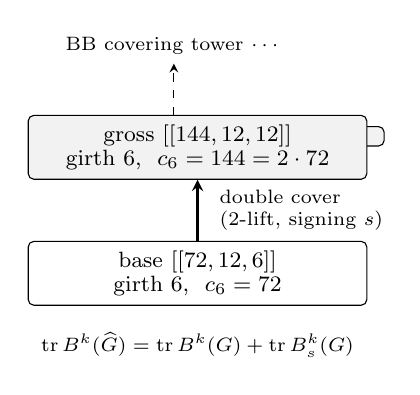
\begin{tikzpicture}[font=\footnotesize,>=stealth,
  box/.style={draw,rounded corners=2pt,align=center,inner sep=3.5pt,minimum width=4.3cm}]
  \node[box] (base) at (0,0) {base $[[72,12,6]]$\\[-1pt]girth 6,\ \ $c_6=72$};
  \node[box,fill=black!5] (covb) at (0.22,1.74) {};
  \node[box,fill=black!5] (cov)  at (0,1.6) {gross $[[144,12,12]]$\\[-1pt]girth 6,\ \ $c_6=144=2\cdot 72$};
  \draw[->,thick] (base.north) -- (cov.south)
    node[midway,right=1.5mm,align=left,font=\scriptsize]{double cover\\($2$-lift, signing $s$)};
  \draw[->,dashed] ([xshift=-3mm]cov.north) -- ++(0,6.5mm)
    node[above,font=\scriptsize]{BB covering tower $\cdots$};
  \node[below=2.2mm of base,font=\scriptsize]
    {$\tr B^k(\widehat G)=\tr B^k(G)+\tr B_s^k(G)$};
\end{tikzpicture}
\caption{The covering-tower factorization. The gross code's Tanner graph is a double cover
($2$-lift) of the $[[72,12,6]]$ graph (two sheets, shown stacked); its certified short-cycle
profile lifts through the signed non-backtracking trace~\eqref{eq:lift}. Girth cycles carry
voltage $+1$, so $c_6$ doubles ($72\!\to\!144$); past the girth the signing is nontrivial
(Table~\ref{tab:lift}).}
\label{fig:cover}
\end{figure}

\begin{table}[t]
\caption{Verification of the $2$-lift factorization~\eqref{eq:lift} on the
gross/$[[72,12,6]]$ pair, in exact arithmetic. The identity holds for every $k$; past the
girth ($k=8$) the signed trace is nontrivial, so the factorization is informative, not a mere
doubling.}
\label{tab:lift}
\centering
\begin{tabular}{@{}lrrr@{}}
\toprule
$k$ & $\tr B^k(\widehat G)$ & $\tr B^k(G)$ & $\tr B_s^k(G)$ \\
\midrule
$1$--$5$ & $0$ & $0$ & $0$ \\
$6$ & $1\,728$ & $864$ & $864$ \\
$7$ & $0$ & $0$ & $0$ \\
$8$ & $27\,648$ & $31\,104$ & $-3\,456$ \\
\bottomrule
\end{tabular}
\end{table}

The clean value $c_6=2\cdot72$ is not a coincidence. BB codes form \emph{covering
towers}~\cite{Symons}: the gross Tanner graph is a \emph{double cover} ($2$-lift) of the
$[[72,12,6]]$ Tanner graph, which we confirm independently (each base edge lifts to exactly one
sheet; $|V(\widehat G)|=2|V(G)|$). For a double cover with edge signing $s$, the
non-backtracking spectrum splits by the classical Artin--Ihara / $2$-lift
identity~\cite{StarkTerras,MSS}:
\begin{equation}
\tr B^k(\widehat G) = \tr B^k(G) + \tr B_s^k(G),
\label{eq:lift}
\end{equation}
where $B_s$ is the \emph{signed} non-backtracking operator of the base. We verify
\eqref{eq:lift} exactly for all $k=1,\dots,8$ on the gross/$[[72,12,6]]$ pair
(Table~\ref{tab:lift}). At the girth, $\tr B^6(\widehat G)=1728=864+864$: every base $6$-cycle
carries voltage $+1$ and lifts to two cover $6$-cycles, so $c_6$ doubles ($72\to144$). Past the
girth the signing is nontrivial---at $k=8$ the signed trace is $-3456$---so the cover's
longer-cycle structure genuinely differs from its base. Consequently the certified short-cycle
profile of a BB \emph{code family} is determined by its base together with the covering
signing, through the Artin--Ihara $L$-function factorization (Fig.~\ref{fig:cover})---a
practical handle on whole towers rather than one code at a time.

\section{Discussion: Scope and Guarantees}
\label{sec:honest}
We are deliberately exact about what is and is not certified.

\emph{The certified object is the identity, not each number.} Equation~\eqref{eq:gaplaw} is
machine-checked for \emph{all} finite graphs~\cite{PartVI}. A per-code count such as $c_6=144$
is a computation; its trustworthiness comes from three independent routes agreeing and from the
theorem-mandated below-girth vanishing being observed, not from a per-code kernel certificate.
We note plainly that neither a cross-check nor a proof assistant validates that the input graph
is the intended code---that is a provenance question---so we do not describe the per-code counts
as ``kernel-checked.''

\emph{No new mathematics.} The gap law is classical and folklore-adjacent; the BB covering
construction is~\cite{Symons}; the $2$-lift factorization is classical~\cite{StarkTerras,MSS}.
The contribution is the methodology (a theorem-backed identity, cross-validated outputs,
reproducible open scripts) and its transfer to deployed classical and quantum codes.

\emph{Relation to distance certificates.} The load-bearing certificate of a quantum code's
strength is its \emph{distance}, machine-checked by Lean-QEC~\cite{LeanQEC} via a verified SAT
reduction. The present diagnostic is decoder-facing and complementary: distance bounds what the
code can correct in principle; the short-cycle profile concerns the practical BP decoder.

\emph{What it does not reach.} The error-floor structures past the girth (trapping and
absorbing sets) are not addressed; we count shortest cycles, the entry-level diagnostic.

\section{Open Questions}
\label{sec:open}
We leave four questions, in increasing reach, for others to take up.
\begin{enumerate}
\item \emph{The corrected window.} The gap law is exact for $k\le g+1$; engineers count to
$2g-2$ with correction terms~\cite{Blake}. What walk family does the $k=g+2$ defect
$\tr A^k-p_k-\tr B^k$ count, and can the corrected multiplicities be given a theorem-backed
form?
\item \emph{The tower as a design principle.} The short-cycle profile factorizes across a BB
cover through the signed trace~\eqref{eq:lift}. Can the covering signing be \emph{chosen} to
suppress the short-cycle population---or raise the girth---at every level of the tower, turning
the factorization from a diagnostic into a construction rule?
\item \emph{From cycles to expansion.} The decoder-relevant quantity for expander-based qLDPC
codes is the spectral gap (the Ramanujan property), set by the leading non-backtracking
eigenvalue. How tightly do the certified low moments $\tr B^g$ and $\tr B^{g+1}$ bound that
gap, and hence the BP threshold?
\item \emph{Beyond shortest cycles.} The error floor is governed by trapping and absorbing
sets, not by the girth alone. Is there a trace-formula-style identity that certifies the
smallest such sets, extending the present diagnostic from the entry level to the structures
that actually limit performance?
\end{enumerate}

\section{Conclusion}
We have presented a short-cycle diagnostic for LDPC Tanner graphs whose defining identity is a
machine-checked theorem and whose outputs are validated by three independent routes, applied to
the deployed IEEE~802.11n codes and, for the first time to our knowledge, to a deployed quantum LDPC code, with a
covering-tower factorization that lifts the profile across a BB code family. The same pipeline
applies to the 3GPP~5G~NR base graphs and to larger BB towers; certifying spectral expansion
(the Ramanujan property), which governs distance and decoding for expander-based qLDPC codes, is
an active research direction to which the formalized non-backtracking and matching-polynomial
machinery used here is naturally suited.

\section*{Reproducibility}
The code constructions, the three-route census and the double-cover factorization check are
open at \url{https://github.com/karlesmarin/godsil-gutman-lean} (\texttt{research/qldpc-gross/}
and the IEEE~802.11n census), together with the Lean~4 sources that prove identity
\eqref{eq:gaplaw}.

\section*{Acknowledgment}
The author used Claude (Anthropic), a large language model, as a computational and drafting
assistant. Under the author's direction it generated and executed the cycle-census and
covering-factorization scripts whose outputs appear in Sections~\ref{sec:wifi}--\ref{sec:cover}
and Tables~\ref{tab:wifi}--\ref{tab:lift}, and it assisted in drafting and editing the text.
The underlying identity~\eqref{eq:gaplaw} is established by a proof-assistant kernel and each
reported count is established by three independent cross-checks; the AI generated neither
guarantee. All mathematics, the choice and interpretation of results, and all claims are the
author's responsibility.

\begin{thebibliography}{99}
\bibitem{Gallager} R.~G. Gallager, ``Low-density parity-check codes,'' \emph{IRE Trans. Inf.
Theory}, vol.~8, no.~1, pp.~21--28, 1962.
\bibitem{Tanner} R.~M. Tanner, ``A recursive approach to low complexity codes,'' \emph{IEEE
Trans. Inf. Theory}, vol.~27, no.~5, pp.~533--547, 1981.
\bibitem{Karimi} M. Karimi and A.~H. Banihashemi, ``Message-passing algorithms for counting
short cycles in a graph,'' \emph{IEEE Trans. Commun.}, vol.~61, no.~2, pp.~485--495, 2013.
\bibitem{Blake} I.~F. Blake and S. Lin, ``On short cycle enumeration in biregular bipartite
graphs,'' \emph{IEEE Trans. Inf. Theory}, vol.~64, no.~10, pp.~6526--6535, 2018.
\bibitem{Bravyi} S. Bravyi \emph{et al.}, ``High-threshold and low-overhead fault-tolerant
quantum memory,'' \emph{Nature}, vol.~627, pp.~778--782, 2024. arXiv:2308.07915.
\bibitem{Symons} B.~C.~B. Symons, A. Rajput, and D.~E. Browne, ``Sequences of bivariate bicycle
codes from covering graphs,'' 2025. arXiv:2511.13560.
\bibitem{LeanQEC} M. Ehatamm, Y. Lee, X. Wu, and R. Tao, ``End-to-end formalization of quantum
error correction,'' 2026. arXiv:2605.16523.
\bibitem{StarkTerras} H.~M. Stark and A. Terras, ``Zeta functions of finite graphs and
coverings, II,'' \emph{Adv. Math.}, vol.~154, no.~1, pp.~132--195, 2000.
\bibitem{MSS} A. Marcus, D.~A. Spielman, and N. Srivastava, ``Interlacing families I: bipartite
Ramanujan graphs of all degrees,'' \emph{Ann. of Math.}, vol.~182, no.~1, pp.~307--325, 2015.
\bibitem{PartVI} C. Mar\'in, ``The walks that remember the cycles: a machine-checked sharp gap
law between the matching polynomial and the non-backtracking spectrum in Lean~4,'' Zenodo,
2026, doi:10.5281/zenodo.20648488.
\end{thebibliography}

\end{document}
